% Editable source for lookup_diagnosis.pdf, written by make_figures.py from analysis/profile_local.json
\documentclass[border=6pt]{standalone}
\usepackage{tikz}
\begin{document}
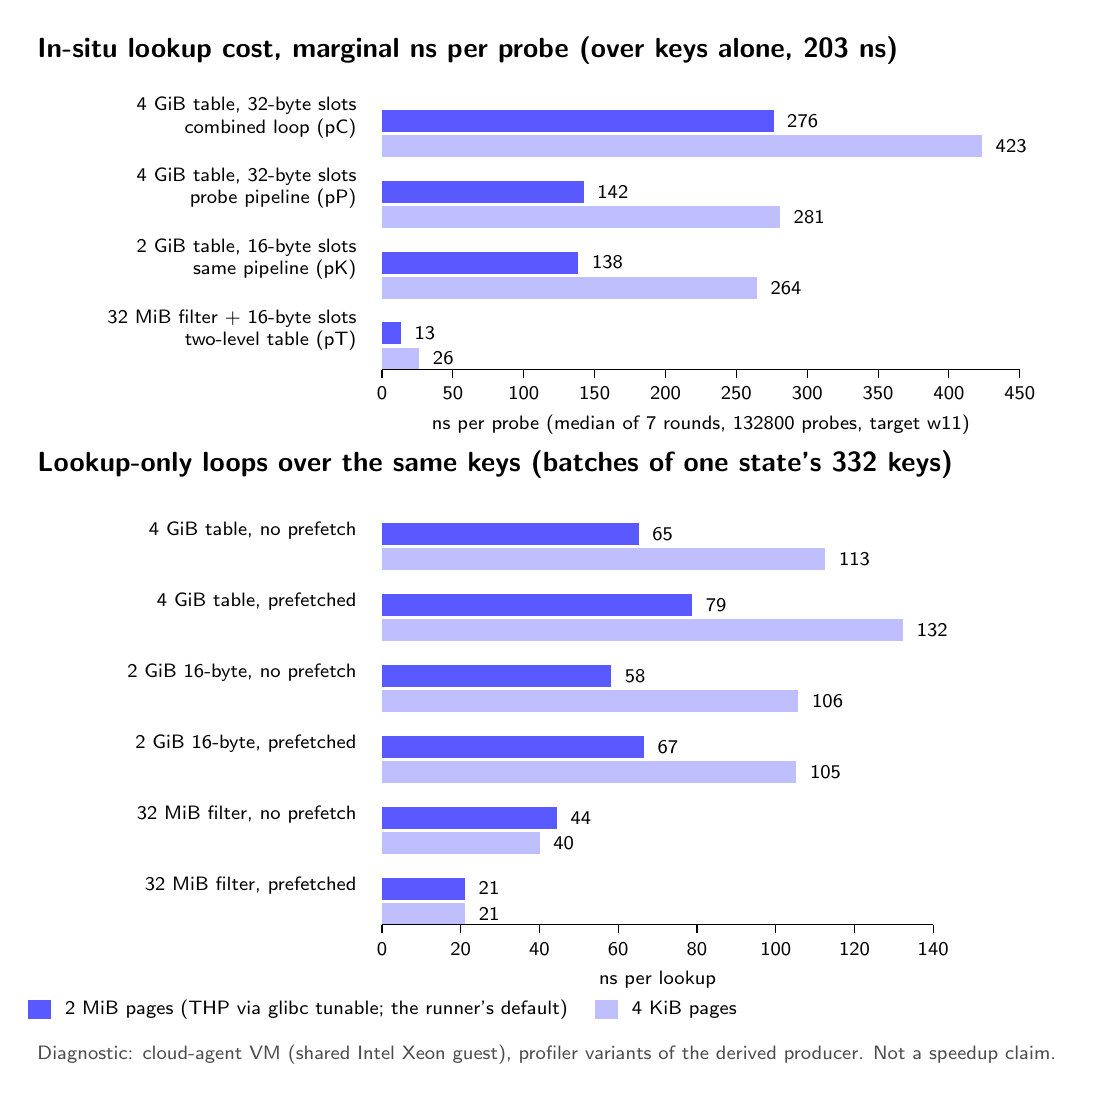
\begin{tikzpicture}[font=\sffamily\small]
\node[anchor=west,font=\sffamily\bfseries] at (0.00,0.00) {In-situ lookup cost, marginal ns per probe (over keys alone, 203 ns)};
\node[anchor=east,align=right,font=\sffamily\scriptsize] at (4.30,-0.85) {4 GiB table, 32-byte slots\\combined loop (pC)};
\fill[blue!65] (4.500,-0.75) rectangle (9.472,-1.03);
\node[anchor=west,font=\sffamily\scriptsize] at (9.522,-0.89) {276};
\fill[blue!25] (4.500,-1.07) rectangle (12.120,-1.35);
\node[anchor=west,font=\sffamily\scriptsize] at (12.170,-1.21) {423};
\node[anchor=east,align=right,font=\sffamily\scriptsize] at (4.30,-1.75) {4 GiB table, 32-byte slots\\probe pipeline (pP)};
\fill[blue!65] (4.500,-1.65) rectangle (7.062,-1.93);
\node[anchor=west,font=\sffamily\scriptsize] at (7.112,-1.79) {142};
\fill[blue!25] (4.500,-1.97) rectangle (9.555,-2.25);
\node[anchor=west,font=\sffamily\scriptsize] at (9.605,-2.11) {281};
\node[anchor=east,align=right,font=\sffamily\scriptsize] at (4.30,-2.65) {2 GiB table, 16-byte slots\\same pipeline (pK)};
\fill[blue!65] (4.500,-2.55) rectangle (6.993,-2.83);
\node[anchor=west,font=\sffamily\scriptsize] at (7.043,-2.69) {138};
\fill[blue!25] (4.500,-2.87) rectangle (9.261,-3.15);
\node[anchor=west,font=\sffamily\scriptsize] at (9.311,-3.01) {264};
\node[anchor=east,align=right,font=\sffamily\scriptsize] at (4.30,-3.55) {32 MiB filter + 16-byte slots\\two-level table (pT)};
\fill[blue!65] (4.500,-3.45) rectangle (4.740,-3.73);
\node[anchor=west,font=\sffamily\scriptsize] at (4.790,-3.59) {13};
\fill[blue!25] (4.500,-3.77) rectangle (4.973,-4.05);
\node[anchor=west,font=\sffamily\scriptsize] at (5.023,-3.91) {26};
\draw (4.50,-4.05) -- (12.600,-4.05);
\draw (4.500,-4.05) -- (4.500,-4.15) node[below,font=\sffamily\scriptsize] {0};
\draw (5.400,-4.05) -- (5.400,-4.15) node[below,font=\sffamily\scriptsize] {50};
\draw (6.300,-4.05) -- (6.300,-4.15) node[below,font=\sffamily\scriptsize] {100};
\draw (7.200,-4.05) -- (7.200,-4.15) node[below,font=\sffamily\scriptsize] {150};
\draw (8.100,-4.05) -- (8.100,-4.15) node[below,font=\sffamily\scriptsize] {200};
\draw (9.000,-4.05) -- (9.000,-4.15) node[below,font=\sffamily\scriptsize] {250};
\draw (9.900,-4.05) -- (9.900,-4.15) node[below,font=\sffamily\scriptsize] {300};
\draw (10.800,-4.05) -- (10.800,-4.15) node[below,font=\sffamily\scriptsize] {350};
\draw (11.700,-4.05) -- (11.700,-4.15) node[below,font=\sffamily\scriptsize] {400};
\draw (12.600,-4.05) -- (12.600,-4.15) node[below,font=\sffamily\scriptsize] {450};
\node[font=\sffamily\scriptsize] at (8.550,-4.75) {ns per probe (median of 7 rounds, 132800 probes, target w11)};
\node[anchor=west,font=\sffamily\bfseries] at (0.00,-5.25) {Lookup-only loops over the same keys (batches of one state's 332 keys)};
\node[anchor=east,align=right,font=\sffamily\scriptsize] at (4.30,-6.10) {4 GiB table, no prefetch};
\fill[blue!65] (4.500,-6.00) rectangle (7.759,-6.28);
\node[anchor=west,font=\sffamily\scriptsize] at (7.809,-6.14) {65};
\fill[blue!25] (4.500,-6.32) rectangle (10.130,-6.60);
\node[anchor=west,font=\sffamily\scriptsize] at (10.180,-6.46) {113};
\node[anchor=east,align=right,font=\sffamily\scriptsize] at (4.30,-7.00) {4 GiB table, prefetched};
\fill[blue!65] (4.500,-6.90) rectangle (8.438,-7.18);
\node[anchor=west,font=\sffamily\scriptsize] at (8.488,-7.04) {79};
\fill[blue!25] (4.500,-7.22) rectangle (11.118,-7.50);
\node[anchor=west,font=\sffamily\scriptsize] at (11.168,-7.36) {132};
\node[anchor=east,align=right,font=\sffamily\scriptsize] at (4.30,-7.90) {2 GiB 16-byte, no prefetch};
\fill[blue!65] (4.500,-7.80) rectangle (7.410,-8.08);
\node[anchor=west,font=\sffamily\scriptsize] at (7.460,-7.94) {58};
\fill[blue!25] (4.500,-8.12) rectangle (9.789,-8.40);
\node[anchor=west,font=\sffamily\scriptsize] at (9.839,-8.26) {106};
\node[anchor=east,align=right,font=\sffamily\scriptsize] at (4.30,-8.80) {2 GiB 16-byte, prefetched};
\fill[blue!65] (4.500,-8.70) rectangle (7.826,-8.98);
\node[anchor=west,font=\sffamily\scriptsize] at (7.876,-8.84) {67};
\fill[blue!25] (4.500,-9.02) rectangle (9.762,-9.30);
\node[anchor=west,font=\sffamily\scriptsize] at (9.812,-9.16) {105};
\node[anchor=east,align=right,font=\sffamily\scriptsize] at (4.30,-9.70) {32 MiB filter, no prefetch};
\fill[blue!65] (4.500,-9.60) rectangle (6.722,-9.88);
\node[anchor=west,font=\sffamily\scriptsize] at (6.772,-9.74) {44};
\fill[blue!25] (4.500,-9.92) rectangle (6.503,-10.20);
\node[anchor=west,font=\sffamily\scriptsize] at (6.553,-10.06) {40};
\node[anchor=east,align=right,font=\sffamily\scriptsize] at (4.30,-10.60) {32 MiB filter, prefetched};
\fill[blue!65] (4.500,-10.50) rectangle (5.554,-10.78);
\node[anchor=west,font=\sffamily\scriptsize] at (5.604,-10.64) {21};
\fill[blue!25] (4.500,-10.82) rectangle (5.555,-11.10);
\node[anchor=west,font=\sffamily\scriptsize] at (5.605,-10.96) {21};
\draw (4.50,-11.10) -- (11.500,-11.10);
\draw (4.500,-11.10) -- (4.500,-11.20) node[below,font=\sffamily\scriptsize] {0};
\draw (5.500,-11.10) -- (5.500,-11.20) node[below,font=\sffamily\scriptsize] {20};
\draw (6.500,-11.10) -- (6.500,-11.20) node[below,font=\sffamily\scriptsize] {40};
\draw (7.500,-11.10) -- (7.500,-11.20) node[below,font=\sffamily\scriptsize] {60};
\draw (8.500,-11.10) -- (8.500,-11.20) node[below,font=\sffamily\scriptsize] {80};
\draw (9.500,-11.10) -- (9.500,-11.20) node[below,font=\sffamily\scriptsize] {100};
\draw (10.500,-11.10) -- (10.500,-11.20) node[below,font=\sffamily\scriptsize] {120};
\draw (11.500,-11.10) -- (11.500,-11.20) node[below,font=\sffamily\scriptsize] {140};
\node[font=\sffamily\scriptsize] at (8.000,-11.80) {ns per lookup};
\fill[blue!65] (0,-12.30) rectangle ++(0.3,0.25); \node[anchor=west,font=\sffamily\scriptsize] at (0.35,-12.18) {2 MiB pages (THP via glibc tunable; the runner's default)};
\fill[blue!25] (7.2,-12.30) rectangle ++(0.3,0.25); \node[anchor=west,font=\sffamily\scriptsize] at (7.55,-12.18) {4 KiB pages};
\node[anchor=west,font=\sffamily\scriptsize,text=black!70] at (0,-12.75) {Diagnostic: cloud-agent VM (shared Intel Xeon guest), profiler variants of the derived producer. Not a speedup claim.};
\end{tikzpicture}
\end{document}
